\documentclass{report}

%%METADATA
\title{Menu Cost Models}
\author{
Raman Singh Chhina \\ {University of Chicago}
}
\date{}

%%PACKAGES
\usepackage{graphicx}
\usepackage{tabularx}
\usepackage{setspace}
\usepackage{amsmath,amsthm,amssymb}
\usepackage[hyphens]{url}
\usepackage{natbib}
\usepackage[font=normalsize,labelfont=bf]{caption}
\usepackage[margin=1in]{geometry}
\usepackage{hyperref}
\hypersetup{colorlinks=true,urlcolor=blue,citecolor=red}
\usepackage{enumerate}% http://ctan.org/pkg/enumerate %Supports lowercase Roman-letter enumeration
\usepackage{verbatim} %Package with \begin{comment} environment
\usepackage{physics}
\usepackage{tikz}
\usepackage{listings}
\usepackage{upquote}
\usepackage{booktabs} %Package with \toprule and \bottomrule
\usepackage{etoc}     %Package with \localtableofcontents
\usepackage{multicol}
\usepackage{bm}
\usepackage{float}

\definecolor{dkgreen}{rgb}{0,0.6,0}
\definecolor{gray}{rgb}{0.5,0.5,0.5}
\definecolor{mauve}{rgb}{0.58,0,0.82}

\lstset{language=bash,
  frame=tb,
  aboveskip=3mm,
  belowskip=3mm,
  showstringspaces=false,
  columns=flexible,
  basicstyle={\small\ttfamily},
  numbers=none,
  numberstyle=\tiny\color{gray},
  keywordstyle=\color{blue},
  commentstyle=\color{dkgreen},
  stringstyle=\color{mauve},
  breaklines=true,
  breakatwhitespace=false,
  tabsize=3
}



%%FORMATTING
\onehalfspacing
\numberwithin{equation}{section}
\numberwithin{figure}{section}
\numberwithin{table}{section}
\bibliographystyle{bib/aeanobold-oxford.bst}

%LOGBOOK
\begin{document}

%%LOGBOOK COVER
\maketitle

%TABLE OF CONTENTS
\renewcommand{\thechapter}{\Alph{chapter}}
\setcounter{tocdepth}{1}
\tableofcontents
\etocsettocstyle{}{} % from now on only local tocs

%%LOGBOOK ENTRIES: Call notes
%\chapter{The Model}This is a model in which firms decide their prices when they are subjected to menu costs. There are aggregate shocks as well as idiosyncratic shocks to the firms productivities. The introduction of the paper is really good and should be read everytime you want to referesh this paper. Here is the \href{https://www.jstor.org/stable/pdf/10.1086/512625.pdf?casa_token=RizjOY_F_XwAAAAA:BCyyclp2TThp916QIcim9m915PciFhUa_3nctyOocZTTXWTaCuUhA5i01fCoI3WF7fZ4wntxRfGwKfsJI0NpS3lNyLzxs7hzvctl66z-1rL8p_0lJjM}{link}. \\

This paper was taught by Fernando as well as Joe, so together it should be covered quite comprehensively. I will first setup the model as in Fernando's class and then go through the code to solve it.

\section{Continuous Time Setup}

``\textit{The theory that we calibrate and simulate in this paper is a Bellman
equation for a single price-setting firm that hires labor at a given nominal
wage, produces a consumption good with a stochastically varying tech nology, and sets product price subject to a menu cost of repricing. We
situate our model of a firm in a model of a monetary economy so as
to be able to relate its predictions to aggregative evidence. In this economy, there is a continuum of infinitely lived households, each of which
consumes a continuum of goods. A Spence-Dixit-Stiglitz utility function
is used to aggregate across goods to form current-period utility. Each
household also supplies labor on a competitive labor market. Firms hire
labor, used to produce the consumption good and to reset nominal
prices for the good, and sell goods to consumers. Each firm produces
only one of the continuum of consumption goods. The economy is subject to two kinds of shocks: a monetary shock,
which we summarize in the money supply $m_t$ , and a firm-specific pro- mt
ductivity shock $\nu_t$ .}''

\subsection{Households}

The households solve the following problem

\begin{align}
  \max_{l(t), c_{ki}(t), M(t)} \int_0^{\infty} \left[ \frac{c(t)^{1-\epsilon_c}}{1-\epsilon_c} - \frac{\alpha}{1+\epsilon_l} l(t)^{1+\epsilon_l} + \log \left( \frac{M(t)}{P(t)} \right)\right] dt \\
  s.t. \\
  0 = M(0) + \int_0^{\infty} Q(t) \left[ \bar \Pi(t) + \tau(t) + (1+\tau_l) W(t) l(t) - R(t)M(t) - \int_0^1 P_k(t)c_k(t) dk \right] dt
\end{align}

i.e. the household maximizes it's lifetime utility — which it gets from consumption, leisure and holding real balances — subject to an aggregate budget constraint. Here $R(t)$ and $W(t)$ are the nominal interest rates and wages respectively. To calculate present values $Q_t$ is defined as $Q_t = \exp \left( - \int_0^t R(s)ds \right)$. In addition to the share in aggregate profits and wage income (which is taxed at the rate $\tau_l$), the households also recieve nominal transfers $\tau(t)$ each period. \\


\textbf{Aside: A note Present Values}

\begin{align}
  PV = FV e^{- rt} \\
  \implies FV = e^{rt} PV
\end{align}

So, the present value increases exponentially due to continuus compounding. The present value of a stream instead is given by

\begin{align}
  PV = \int_0^{\infty} e^{-rt} s(t) dt
\end{align}

and if the interest rates are changing then
\begin{align}
  PV = \int_0^{\infty} e^{- \int_0^t r(s)ds} s(t) dt
\end{align}

\begin{centering}
  *****
\end{centering}

We want to solve for the path of nominal interest rates and wages as functions of the money supply to solve for the equilibrium.
\\

The First order conditions of the problem give us

\begin{align}
  l(t) : 0 = e^{- \rho t} \alpha l(t)^{\epsilon_l} - \lambda_0 (1+\tau_l) Q(t) W(t) \\
  M(t) : 0 = e^{- \rho t} \frac{1}{M(t)} - \lambda_0 Q(t) R(t) \\
  c(t) : 0 = e^{- \rho t} c(t)^{- \epsilon_c} - \lambda_0 Q(t) P(t) \\
  c_k(t): 0 = e^{- \rho t} c(t)^{- \epsilon_c} c(t)^{\frac{1}{\epsilon_m}} c_k(t)^{-\frac{1}{\epsilon_m}} A_k(t)^{\frac{1}{\epsilon_m}} - \lambda_0 Q(t)P_k(t)
\end{align}

Take the FOC w.r.t $M(t)$ first, we have

\begin{align} \label{moneyfoc}
  e^{- \rho t} \frac{1}{M(t)} - \lambda_0 Q(t) R(t)  = 0 \\
  - \rho t - \log M(t) - \log \lambda_0 Q(t) - \log R(t) = 0 && \text{ taking logs } \\
  - \rho - \frac{\dot M (t)}{M(t)} - \frac{\dot Q (t)}{Q(t)} - \frac{\dot R (t)}{R(t)} =  0
\end{align}

\textbf{Assume that the money supply $M(t)$ is growing at a constant rate $\mu$}. To calculate the term with $Q(t)$, note that

\begin{align}
  \log Q(t) = \int_0^t R(s)ds \\
  \frac{d \log Q(t)}{t} = R(t)
\end{align}

Plugging this in \ref{moneyfoc} we get

\begin{align}
  - \rho - \mu - R(t)  - \frac{\dot R (t)}{R(t)} = 0 \\
  \dot R(t) = R(t) (R(t) - \mu - \rho)
\end{align}

One of the solutions of this FOC is
\begin{align}
  R(t) = \mu + \rho
\end{align}
Pluging this back in the FOc we get that
\begin{align}
  \lambda_0 = \frac{1}{M(0)R}
\end{align}
Now, furth`er \textbf{assume that the utility is linear in labor i.e. $\epsilon_l = 0$}. This gives the labor FOC as

\begin{align}
   e^{- \rho t} \alpha  - \lambda_0 (1+\tau_l) Q(t) W(t) = 0 \\
   W(t) = \frac{ e^{- \rho t} \alpha M(0)R}{Q(t) (1+\tau_l)}
\end{align}

using $R(t) = \rho + \mu$

\begin{align}
   W(t) = \frac{ e^{- \rho t} \alpha M(0)R}{e^{ - (\rho - \mu)t} (1+\tau_l)} \\
   W(t) = \frac{\alpha}{1+\tau_l} R M(t)
\end{align}

In the general case, we instead get that

  \begin{align}
     W(t) = l(t)^{\epsilon_l} \frac{\alpha}{1+\tau_l} R M(t) \\
     \text{equivalently} \\
     \log W(t) = \epsilon_l l(t) + \log \left( \frac{\alpha}{1+\tau_l} \right) + \log R + \log M
  \end{align}

Now take the FOC for $c_k(t)$

\begin{align}
   e^{- \rho t} c(t)^{- \epsilon_c} c(t)^{\frac{1}{\epsilon_m}} c_k(t)^{-\frac{1}{\epsilon_m}} A_k(t)^{\frac{1}{\epsilon_m}} = \lambda_0 Q(t)P_k(t) \\
   c_k(t)^{\frac{-1}{\epsilon_m}} = e^{\rho t} c(t)^{\frac{\epsilon_c \epsilon_m - 1}{\epsilon_m}} A_k(t)^{\frac{-1}{\epsilon_m}} \left( \lambda_0 Q(t)P_k(t) \right)
\end{align}

using the fact $Q(t) = \frac{ e^{- \rho t} \alpha M(0)R}{W(t) (1+\tau_l)}$, we get

\begin{align}
  c_k(t)^{\frac{-1}{\epsilon_m}} = e^{\rho t} c(t)^{\frac{\epsilon_c \epsilon_m - 1}{\epsilon_m}} A_k(t)^{\frac{-1}{\epsilon_m}} \left( \lambda_0  \frac{ e^{- \rho t} \alpha M(0)R}{W(t) (1+\tau_l)}P_k(t) l(t)^{-\epsilon_l} \right) \\
  c_k(t) =  c(t)^{1-\epsilon_c \epsilon_m} A_k(t) \left(   \frac{ \alpha P_k(t) }{W(t) (1+\tau_l)} l(t)^{-\epsilon_l} \right)^{- \epsilon_m}
\end{align}

\textbf{Firm profits}: As each firm produces a differentiated variety the profit of the firm is given by

\begin{align}
  P_k(t) c_k(t) - w(t) l(t)
\end{align}

We know that the production technology is linear i.e. $c_k(t) = \frac{l_k(t)}{Z_k(t)}$. Using this we get

\begin{align}
  P_k(t) c_k(t) - w(t) c_k(t) Z_k(t) \\
  c_k(t) \left[ P_k(t) - w_t Z_k(t) \right]
\end{align}

plug in $c_k(t)$ from the household optimization
\begin{align}
c(t)^{1-\epsilon_c \epsilon_m} A_k(t) \left(   \frac{ \alpha P_k(t) }{W(t) (1+\tau_l)} l(t)^{-\epsilon_l} \right)^{- \epsilon_m}  \left[ P_k(t) - w_t Z_k(t) \right]
\end{align}

Discounting we get that

\begin{align}
  \Pi(t) =  Q(t)c(t)^{1-\epsilon_c \epsilon_m} A_k(t) \left(   \frac{ \alpha P_k(t) }{W(t) (1+\tau_l)} l(t)^{-\epsilon_l} \right)^{- \epsilon_m}  \left[ P_k(t) - w_t Z_k(t) \right]
\end{align}


\section{Karan's notes}


\section{Golosov-Lucas in discrete time}

\subsubsection*{Households}
\begin{align*}
    & \max_{{n_t, c_t^i}_t} E_0 \left[ \sum_t \beta^t (\log C_t - \omega n_t) \right]\\
    \text{s.t.} \ & \int_0^1 p_t^ic_t^i \ di \leq W_t n_t + \int_0^1 \pi_t^i\\
    & C_t = \left( \int_0^1 (c_t^i)^{\frac{\theta - 1}{\theta}} \ di\right)^{\frac{\theta}{\theta - 1}}.
\end{align*}
Household demand is therefore,
\begin{align*}
     c_t^i = \left( \frac{p_t^i}{P_t}\right)^{-\theta} C_t, &&
    \text{where} \  P_t = \left( \int_0^1 (p_t^i)^{1-\theta} \ di\right)^{\frac{1}{1 - \theta}}.
\end{align*}
Consumption-leisure tradeoff gives,
\begin{align*}
    \frac{W_t}{P_t} = \omega C_t.
\end{align*}

\subsubsection*{Firms}
\begin{align*}
    & \max_{p^i_t} E_t \left[ Q_t \pi^i_t \right]\\
    \text{where} \ & \pi^i_t = \left( \frac{p^i_t}{P_t} - \frac{W_t}{z^i_t P_t} \right) \left( \frac{p_t^i}{P_t}\right)^{-\theta} C_t - f \frac{W_t}{P_t} \mathbf{1}_{p^i_t \neq p^i_{t-1}},
\end{align*}
where
\begin{align*}
    \log z^i_t = \rho_z \log ^i_{t-1} + \sigma_z \epsilon^i_t && \epsilon^i_t \sim N(0,1),
\end{align*}
and $Q_t$ are the stochastic discount factors (which if multiplied by the appropriate probabilities to get rid of the expectation become Arrow-Debrue prices).

To compute the discount factor, I can introduce bonds into the household's problem, in which case the budget constraint becomes,
\begin{align*}
    & P_t C_t + P_t B_t \leq W_t n_t + \Pi_t + P_t R_t B_{t-1} \\
    & C_t + B_t \leq \frac{W_t}{P_t}n_t + \frac{\Pi_t}{P_t} + R_t B_{t-1}.
\end{align*}
In the second equation above, I've written the budget constraint in real terms as the entire setup is in real terms (including the firm's problem). Euler equation then gives,
\begin{align*}
    \beta \frac{Pr(s^{t+1})}{Pr(s^t)} R_t(s^t) = \frac{C_{t+1}(s^{t+1})}{C_t(s^t)}.
\end{align*}
If there are not aggregate shocks and we seek the stationary equilibrium, we will have $C_{t+1} = C_t$ and hence $R = \beta^{-}$. Otherwise, the stochastic discount factor is,
\begin{align*}
    \frac{1}{R_t(s^t)} = \beta Pr(s^{t+1} \vert s^t)  \frac{C_t(s^t)}{C_{t+1}(s^{t+1})}.
\end{align*}


\subsection{Solving the equilibrium: Krussel-Smith}
Let the aggregate shock in the economy be $S_t$, where
\begin{align*}
    P_t C_t  = S_t.
\end{align*}
Then,
\begin{align*}
    P_t = \phi(\chi(p_{-}, z), S).
\end{align*}
The firm's problem may be summarised as follows,
\begin{align*}
    v(p_{-}, z; \chi(p_{-}, z), S) &= \max\{ v^a(z; \chi(p_{-}, z), S), v^n(p_{-}, z; \chi(p_{-}, z), S) \}\\
    v^a(z; \chi(p_{-}, z), S) &= \max_p \left( \frac{p}{P} - \frac{\omega \frac{S}{P}}{z} \right) \left(\frac{p}{P}\right)^{-\theta} \frac{S}{P} - f \omega \frac{S}{P} + \beta E_{z, S} \frac{\frac{S}{P}}{\frac{S'}{P'}} V\left(\frac{p}{P'}, \rho_z z + \epsilon; \chi'(p_{-}', z'), S' \right)\\
    v^n(p_{-}, z; \chi(p_{-}, z), S) &= \left(\frac{p_{-}}{P} - \frac{\omega \frac{S}{P}}{z}\right) \left(\frac{p_{-}}{P}\right)^{-\theta} \frac{S}{P} + \beta E_{z, S}  \frac{\frac{S}{P}}{\frac{S'}{P'}} V\left(\frac{p_{-}}{P'}, \rho_z z + \epsilon; \chi'(p_{-}', z'), S' \right),
\end{align*}
where
\begin{align*}
    P = \phi(\chi(p_{-}, z), S) && \chi'(p_{-}', z') = \Gamma(\chi(p_{-}, z), S').
\end{align*}
Note the distinction between $P$ (the price level this period) and $P_{-}$ (the price level in the previous period)
\begin{align*}
    P_{-} = \left(\int p_{-}^{1-\theta} \ \chi(dp_{-}, dz)\right)^{\frac{1}{1-\theta}}.
\end{align*}

Following Krussel-Smith (henceforth KS), assume
\begin{align*}
    P = \phi(\hat \chi (p_{-}, z), S),
\end{align*}
where $\hat \chi$ is a finite set of moments of $\chi$. In particular, I conjecture that aggregate variables can be forecast with a log-linear rule using only the first moment of $\chi$. Since $z$ is idiosyncratic and determined independently of $S$, first note that the distribution $\chi$ is seperable, i.e. $\chi(dp_{-}, dz) = \chi_p(dp_{-}) \chi_z(dz)$. It is easier if we take $p_{-}/S$ to be the state variable rather than $p_{-}$ (which is wlog). Letting $\chi_1 = E\left[ \log \left(\frac{p_{-}}{S}\right)\right]$, I assume that the variance of the idiosyncratic shock is small, and hence, $\left(\frac{p_{-}}{S}\right) \approx \chi_1$. But since $P_{-} \approx p_{-} \int (\mathcal{O(\text{second order})})$, which implies $\log P_{-} \approx \log p_{-}$, and therefore $\left(\frac{P_{-}}{S}\right) \approx \chi_1$. Furthermore, given the small variance of the idiosyncratic shock, I assme that $\hat \chi = \chi_1$ and $\phi$ is linear, i.e.,
\begin{align*}
    \log \left( \frac{P}{S}\right) \approx \gamma_0 + \gamma_1\chi_1.
\end{align*}
Moreover,
\begin{align*}
    C = \frac{S}{P} = e^{-(\gamma_0 + \gamma_1 \chi_1)},
\end{align*}
which implies,
\begin{align*}
    Q = \beta\frac{C}{C'} = \beta\frac{\frac{S}{P}}{\frac{S'}{P'}} = \beta \frac{e^{-(\gamma_0 + \gamma_1 \chi_1)}}{-(\gamma_0 + \gamma_1 \chi_1)}.
\end{align*}
The firm's profit can now be written as,
\begin{align*}
    \pi(p, z; \chi_1) &= \left(\frac{p}{S} - \frac{\omega}{z}\right) \left(\frac{p }{S}\right)^{-\theta} e^{(\gamma_0 + \gamma_1\chi_1)(\theta - 2)}.
\end{align*}
The state variables for the firm have now reduced to $p/S, z, \chi_1$. The LOM of $z$ is exogenous, that of
\begin{align*}
    \log z_+ = \rho_z \log z + \sigma_z \epsilon_z.
\end{align*}
For the aggregate transition, since we have $\chi_1 = \log \frac{P_{-}}{S}$,
\begin{align*}
    \chi_{1+} = \log \frac{P}{S_+} = \log \frac{P}{S} + \log \frac{S}{S_+} = \gamma_0 + \gamma_1 \chi_1 - (\mu_m + \epsilon_m)
\end{align*}


\subsubsection*{Summary}
The firm solves,
\begin{align}
    \label{eq:1}
    v\left( \log \frac{p_-}{S}, \log z; \chi_1 \right) &= \max \left\{v^n\left( \log \frac{p_-}{S}, \log z; \chi_1\right), v^a (\log z; \chi_1) \right\}\\ \label{eq:2}
    v^n\left(\log\frac{p_-}{S}, \log z; \chi_1\right) &= \pi\left( \frac{p_-}{S}, z; \chi_1\right) + \beta E_{\epsilon_z, \epsilon_m} Q v\left( \log \frac{p_-}{S} - (\mu_m + \epsilon_m), \log z_+; \chi_{1+} \right) \\ \label{eq:3}
    v^a\left(\log z; \chi_1\right) &= - f \omega e^{-(\gamma_0 + \gamma_1 \chi_1)} + \max_{\frac{p}{S}} \left\{ \pi\left( \frac{p}{S}, z; \chi_1 \right) + \beta E_{\epsilon_z, \epsilon_m} Q v\left(\log \frac{p}{S} - (\mu + \epsilon_m), \log z_+; \chi_{1+} \right) \right\}\\ \label{eq:4}
    \pi(p, z; \chi_1) &= \left(\frac{p}{S} - \frac{\omega}{z}\right) \left(\frac{p }{S}\right)^{-\theta} e^{(\gamma_0 + \gamma_1\chi_1)(\theta - 2)}\\ \label{eq:5}
    \log z_+ &= \rho_z \log z + \sigma_z \epsilon_z \\ \label{eq:6}
    \chi_{1+} &= \gamma_0 + \gamma_1 \chi_1 - (\mu_m + \epsilon_m) \\ \label{eq:7}
    Q &= \beta e^{\gamma_1(\chi_{1+} - \chi_1)} \\ \label{eq:8}
    \log\left(\frac{\tilde p}{S_+}\right) &= \log\left(\frac{\tilde p}{S}\right) - (\mu_m + \epsilon_m).
\end{align}
Note Eq. \eqref{eq:8} results from the fact that each optimising firm $\frac{\tilde p}{S} = \tilde p\left( \log \frac{p_-}{S}, \log z; \chi_1 \right)$. But next period, due to the money shock $S_+ - S$, the firm's state is actually $\log\left(\frac{\tilde p}{S_+}\right)$ and not $\log\left(\frac{\tilde p}{S}\right)$. Since here $S$ follows a random walk, the appropriate correction is $\mu_m + \epsilon_m$.


\clearpage
\section{Code}

The code for both the exercises can be accessed at the Github repository \href{https://github.com/econ-raman/Menu_Cost_Models}{here}.
\chapter{\cite{golosov2007menu} with aggregate volatility}
\section{Impulse Resonse Function}

The impluse response of the economy to a one grid point nominal shock is shown in Figs~\ref{irf1} and \ref{irf2}. The IRF on impact is 98.5\% in this economy (as a fraction of the nominal shock). The IRF dies out in eight to ten periods but it takes a couple of months for the small variations to die out completely.
\begin{figure}[H]
    \centering
    \begin{minipage}{0.48\textwidth}
        \centering
        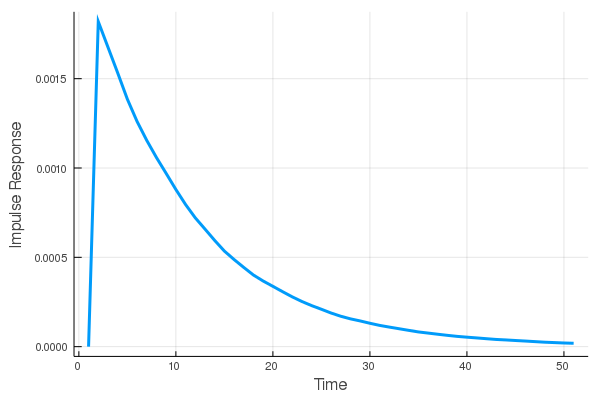
\includegraphics[width = \textwidth]{../tasks/Golosov_lucas/output/C_irf_50_periods.png}
        \caption{IRF till 50 periods after the shock}
        \label{irf1}
    \end{minipage}
    \begin{minipage}{0.48\textwidth}
        \centering
        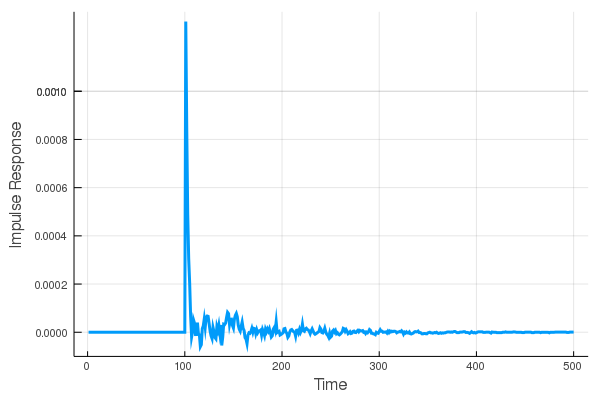
\includegraphics[width=\textwidth]{../tasks/Golosov_lucas/output/C_irf_500_periods.png}
        \caption{IRF for the entire simulation}
        \label{irf2}
    \end{minipage}
\end{figure}

The variance of the output in the baseline economy is . When we double the menu cost from 0.045 to 0.09 the variance of the output increases by 3.038 times.
On doubling the menu cost from 0.045 to 0.09 the variance of output increase by 3.038 times.

\section{Hazard}

The Hazard Function of the economy is as expected from the theory. The firms essentially follow a sS rule and adjust only when the price gaps get more than a certain thresholds. The probability of adjustment is zero within this interval and then jumps immediately to one outside this boundary.
\begin{figure}[H]
    \centering
    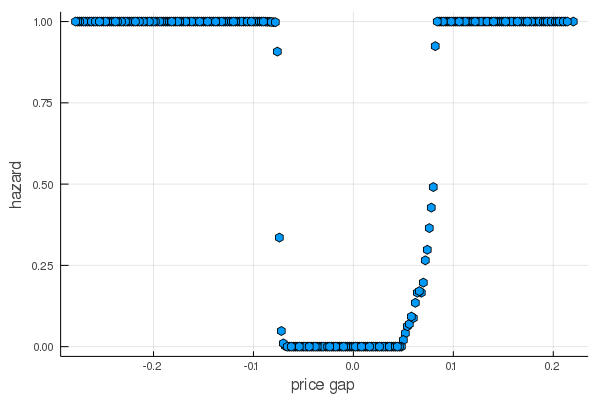
\includegraphics[width = 0.6\textwidth]{../tasks/Golosov_lucas/output/hazard_gl.png}
    \caption{Hazard}
    \label{}
\end{figure}

\section{Price Change Distribution}

Once the firm's price gap gets beyond the inaction interval, they immediately adjust to the optimal. However, due to the presence of aggregate shocks we do not get just the two mass points in the case of standard golosov lucas. Rather we get the distribution as in Fig~\ref{pcgl}.
\begin{figure}[H]
    \centering
    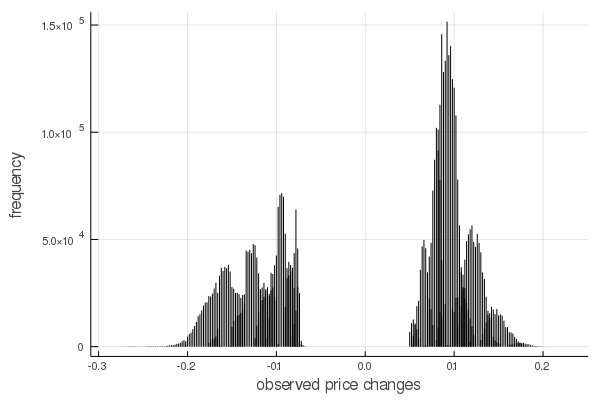
\includegraphics[width = 0.6\textwidth]{../tasks/Golosov_lucas/output/observed_p_changes_gl.png}
    \caption{Observed Price Changes}
    \label{pcgl}
\end{figure}

\section{Ergodic Price Gap Distribution}

In the presence of a positive drift and aggregate shocks to nominal spending, we get the following distribution of the price gaps in the model.
\begin{figure}[H]
    \centering
    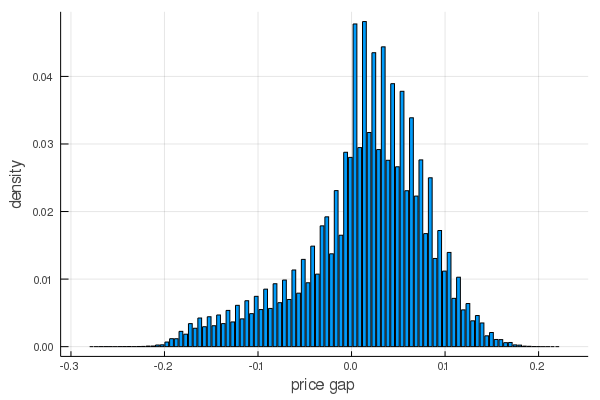
\includegraphics[width = 0.6\textwidth]{../tasks/Golosov_lucas/output/price_gap_dist.png}
    \caption{Price Gap Distribution}
    \label{}
\end{figure}



\chapter{Calvo Plus}\begin{figure}
    \centering
    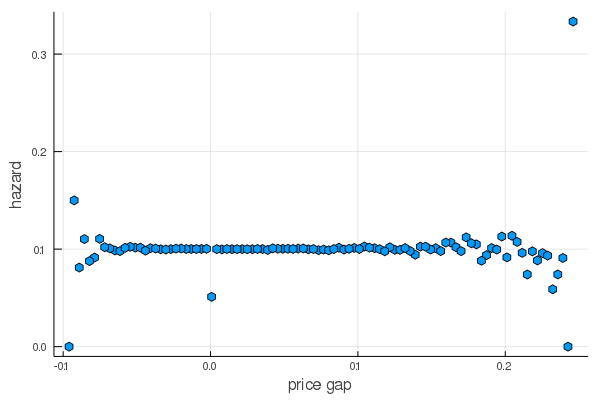
\includegraphics[width = 0.6\textwidth]{../tasks/Calvo_Plus/output/hazard_cp.png}
    \caption{Hazard}
    \label{}
\end{figure}




%%LOGBOOK BIBLIOGRAPHY
\bibliography{bib/reference.bib}

\end{document}
